%%%%%%%%%%%%%%%%%%%%%%%%%%%%%%%%%%%%%%%%%%%%%%%%%%%%%%%%%%%%%%%%%%%%%%
% How to use writeLaTeX: 
%
% You edit the source code here on the left, and the preview on the
% right shows you the result within a few seconds.
%
% Bookmark this page and share the URL with your co-authors. They can
% edit at the same time!
%
% You can upload figures, bibliographies, custom classes and
% styles using the files menu.
%
%%%%%%%%%%%%%%%%%%%%%%%%%%%%%%%%%%%%%%%%%%%%%%%%%%%%%%%%%%%%%%%%%%%%%%

\documentclass[12pt]{article}

\usepackage{sbc-template}

\usepackage{graphicx,url}

% \usepackage[brazil]{babel}   
\usepackage[utf8]{inputenc}  



% pacotes que eu importei
\usepackage{tabularx}
\usepackage{float}
\usepackage{multirow}
\usepackage{booktabs}


     
\sloppy

\title{Exercicio Programa 1}

\author{Pedro Semcovici (12745511) }


\address{Universidade de S\~ao Paulo (EACH-USP) \\ 
	Av Arlindo Bettio 1000, S\~ao Paulo, Brazil 
	\email{pedrosemcovici@usp.br}}

\begin{document} 

\maketitle
     
\begin{resumo} 
Nesse trabalho foi explorado a comparação entre modelo de redes neurais fully connected (FCNN) e redes neurais convolucionais (CNN) para a classificação de imagens do conjunto Kuzushiji-MNIST, que é um conjunto de imagens de 10 possíveis caracteres do Hiragana. Além do experimento básico da comparação entre os dois algoritmos, foi realizado testes removendo a camada de polling da CNN e, também, realizando uma etapa de \textit{data augmentation} em ambos os algoritmos aumentando o conjunto de treino em 10 vezes.
\end{resumo}


\section{Introdução}
Este trabalho trata-se de um exercício programa (EP) da  disciplina MAC5921 - Deep Learning do programa de pós-graduação em Ciência da Computação do IME-USP. A proposta desse trabalho consiste em comparar o desempenho de CNN (Convolucional Neural Network) e FCNN (Fully Connected Neural Network) para a classificação de imagens. Ao longo desse trabalho, serão respondidas algumas das perguntas levantadas no enunciado do trabalho, sendo elas:

\begin{itemize}
  \item Q1 - Como a performance de uma rede neural totalmente conectada se compara com a de uma CNN ao classificar imagens de um dataset específico?
  \item Q2 - Qual é a distribuição das classes no dataset que você escolheu? Existem classes desbalanceadas?
  \item Q3 - Quais são as principais diferenças entre uma rede neural totalmente conectada (fully connected) e uma rede neural convolucional (CNN) em termos de arquitetura?
  \item Q4 - Como as operações de convolução em uma CNN ajudam na extração de características de uma imagem?
  \item Q5 - Qual é o papel das camadas de pooling em uma CNN? Seria possível treinar uma CNN sem elas? O que aconteceria?
  \item Q6 - Como você pode visualizar e interpretar os filtros (kernels) aprendidos por uma CNN?
  \item Q7 - O que essas visualizações dizem sobre o tipo de características que a CNN aprende nas primeiras camadas versus nas últimas?
  \item Q8 - É possível interpretar os pesos de uma rede totalmente conectada da mesma forma? Por que ou por que não?
\end{itemize}





\section{Materiais e Métodos} 

\subsection{Conjunto de dados}

O conjunto de dados utilizado para este trabalho é o Kuzushiji-MNIST \cite{DBLP:journals/corr/abs-1812-01718} disponivel em um repositório do GitHub\footnote{https://github.com/rois-codh/kmnist}. Nesse repositório há a possibilidade de download de 3 datasets (Kuzushiji-MNIST, Kuzushiji-49 e Kuzushiji-Kanji), o escolhido para esse trabalho foi o Kuzushiji-MNIST dado ser o conjunto com a menor quantidade de classes, o que facilita os experimentos. 

O Kuzushiji-MNIST possui um total de 10 classes, sendo cada uma delas um caracter do Hiragana. Uma representação de cada uma das classes pode ser vista abaixo, sendo cada ``linha" uma classe, a primeira ``coluna" sendo um bom exemplo (digital) do caracter e as outras sendo exemplos escritos à mão.

\begin{figure}[ht]
  \centering
  \includegraphics[width=.5\textwidth]{../images/kmnist_examples.png}
  \caption{Exemplos de imagens do Kuzushiji-MNIST}
  \label{fig:kmnist-examples}
\end{figure}

O conjunto de dados já possui uma separação de treino e teste, sendo 60 mil imagens no conjunto de treino e 10 mil no de teste. Além disso, o conjunto é perfeitamente balanceado, possuindo exatamente 10\% das observações para cada uma das classes, sendo assim 6 mil observações para cada classe no treino e mil para o teste.

As imagens do cojunto de dados são de baixa resolução, tendo dimensões (28,28,1). As imagens são disponibilizadas em formato numpy, o que facilita a leitura dos dados.


\subsection{Experimentos realizados}

Os modelos treinados são CNN  e FCNN, além de testar algumas alterações para ver se essas melhoram ou pioram o desempenho. Assim resultando nos seguintes experimentos:

\begin{enumerate}
  \item \textbf{CNN}: modelo CNN simples
  \item \textbf{FCNN}: modelo FCNN simples 
  \item \textbf{CNN com data augmentation}: modelo CNN com dados aumentados em 10x
  \item \textbf{FCNN com data augmentation}: modelo FNN com dados aumentados em 10x
  \item \textbf{CNN sem camada de polling}: modelo CNN removendo a camada de polling
\end{enumerate}

Os modelos CNN e FCNN seguem as estruturas demonstradas na Figuras \ref{fig:model_cnn_graph} e \ref{fig:model_fcnn_graph}, respectivamente. Tendo apenas a mudança de retirar a camada de max\_polling2d no caso do experimento ``CNN sem camadda de polling".


\begin{figure}[H]
  \centering
  \begin{minipage}{0.4\textwidth}
    \centering
    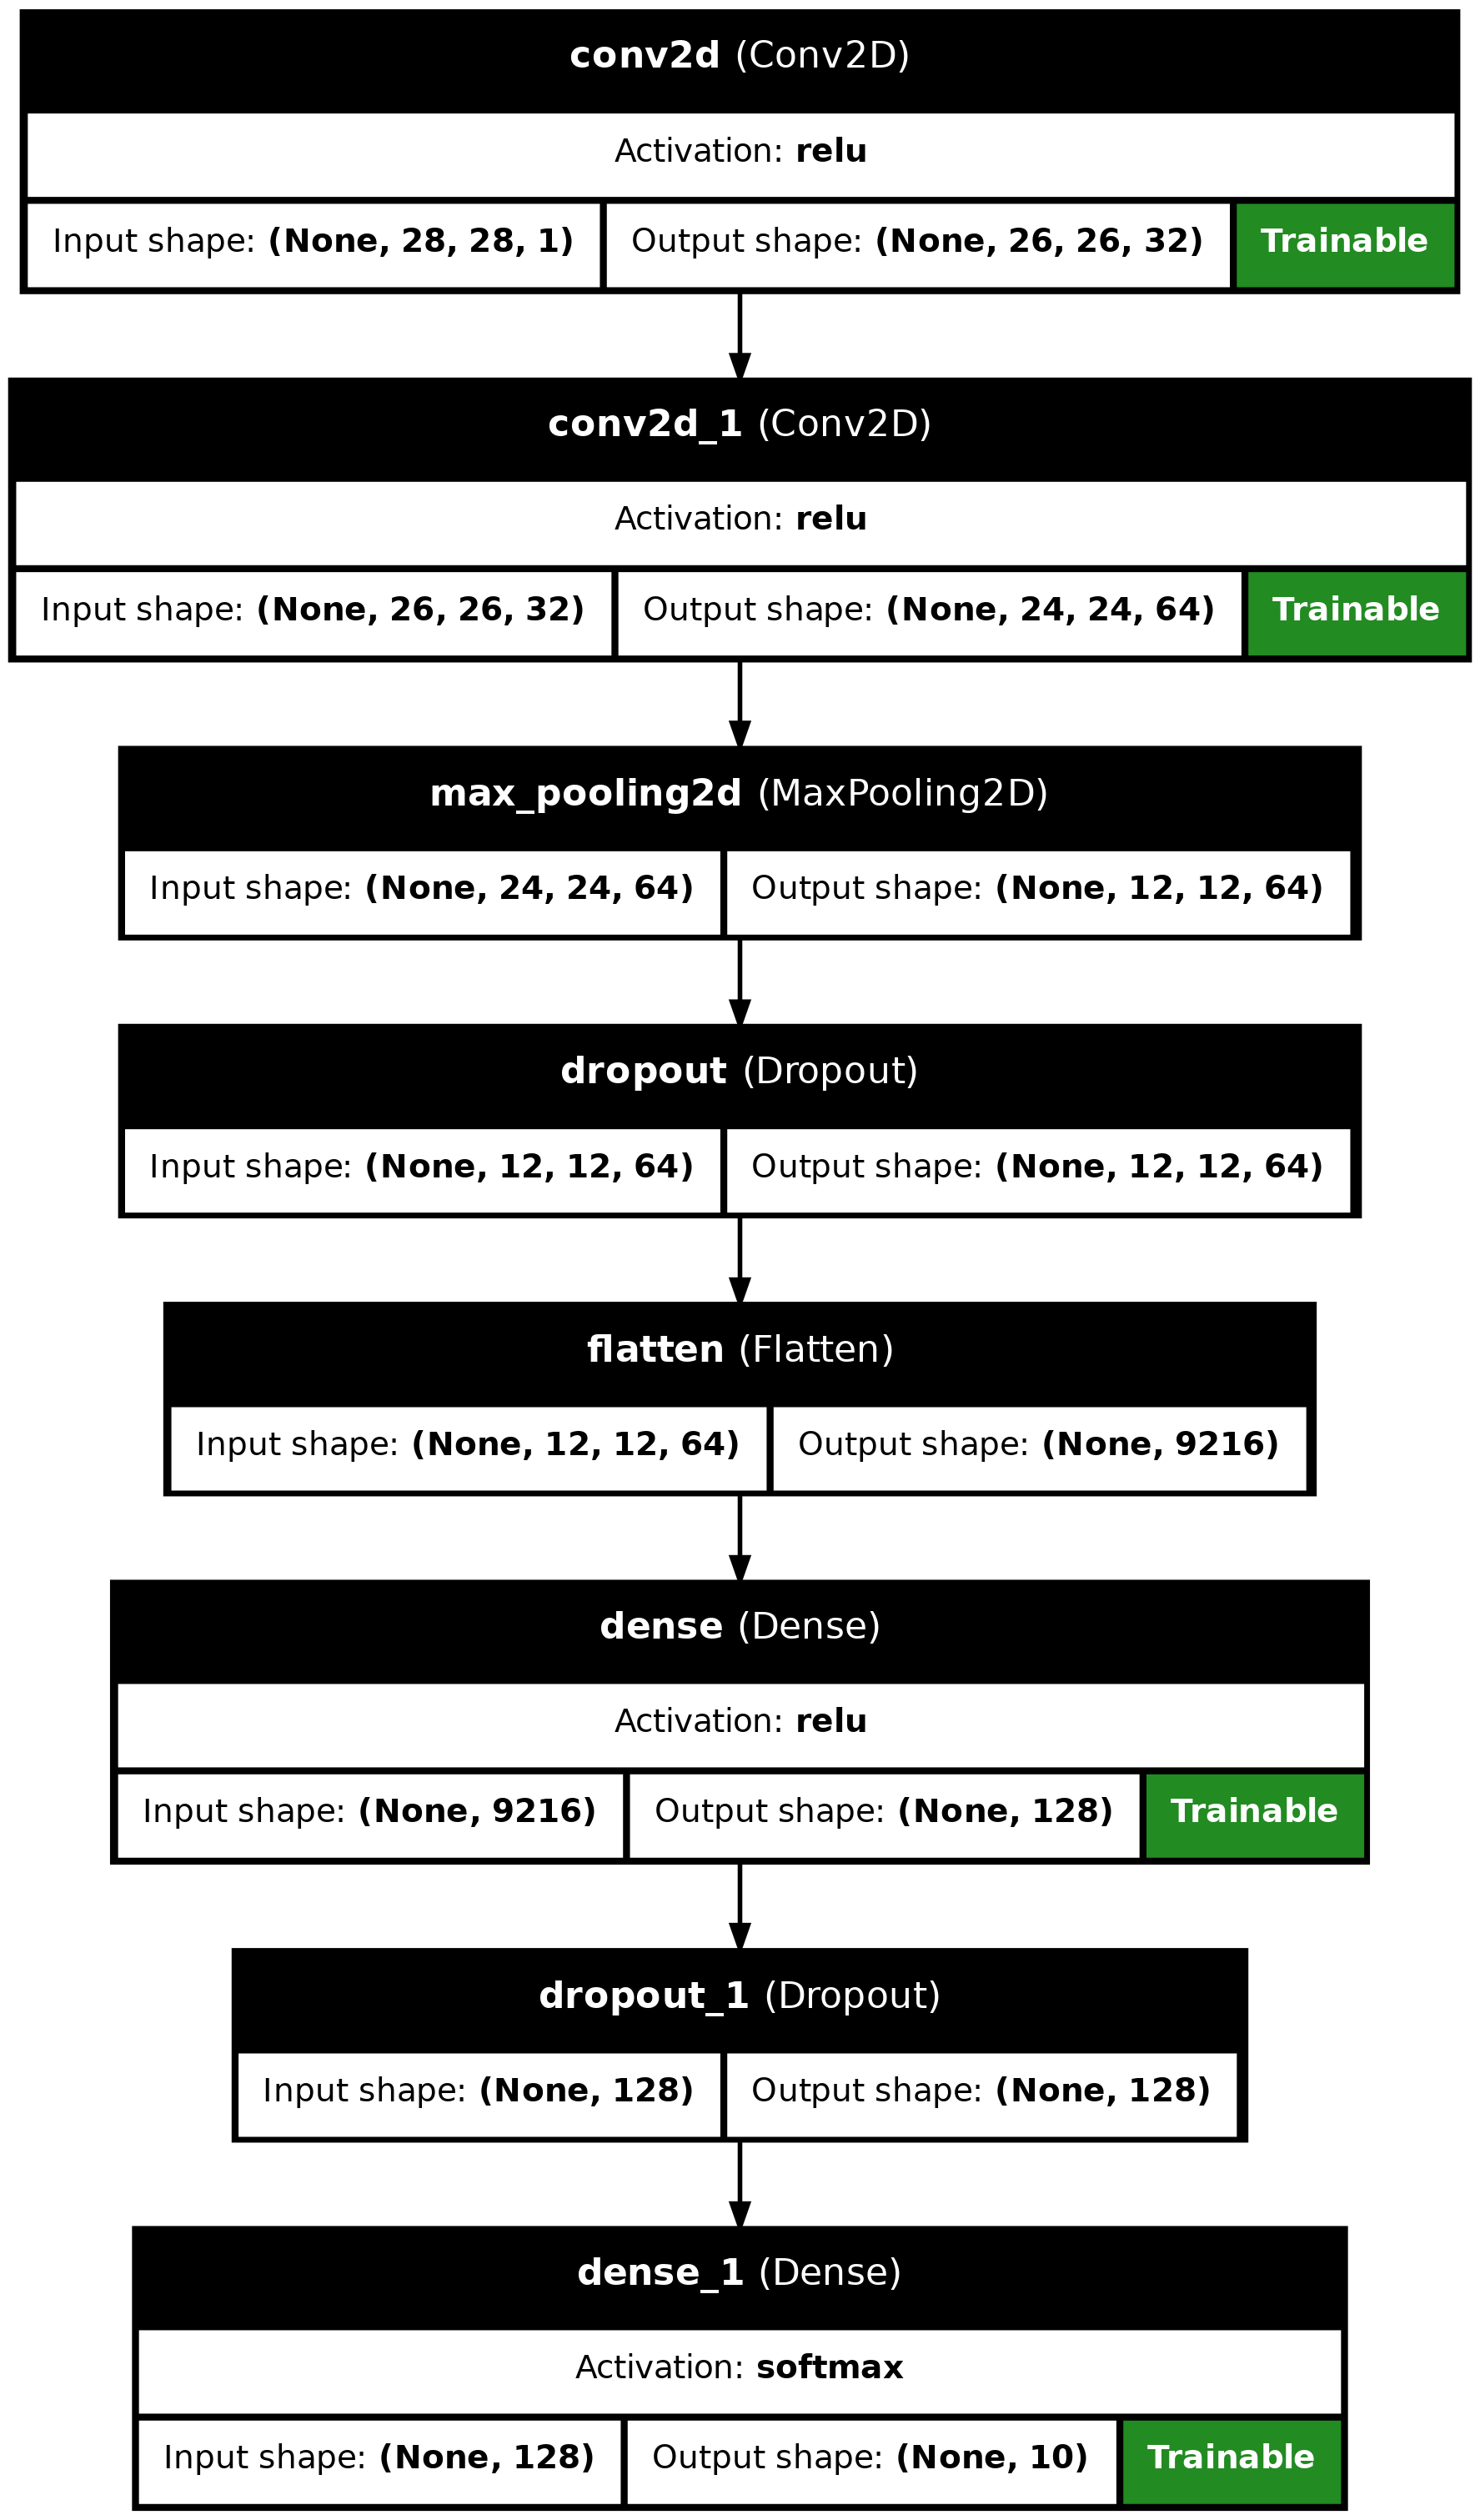
\includegraphics[width=\textwidth]{../images/models/model_cnn_graph.png}
    \caption{Model CNN}
    \label{fig:model_cnn_graph}
  \end{minipage}%
  \hfill
  \begin{minipage}{0.4\textwidth}
    \centering
    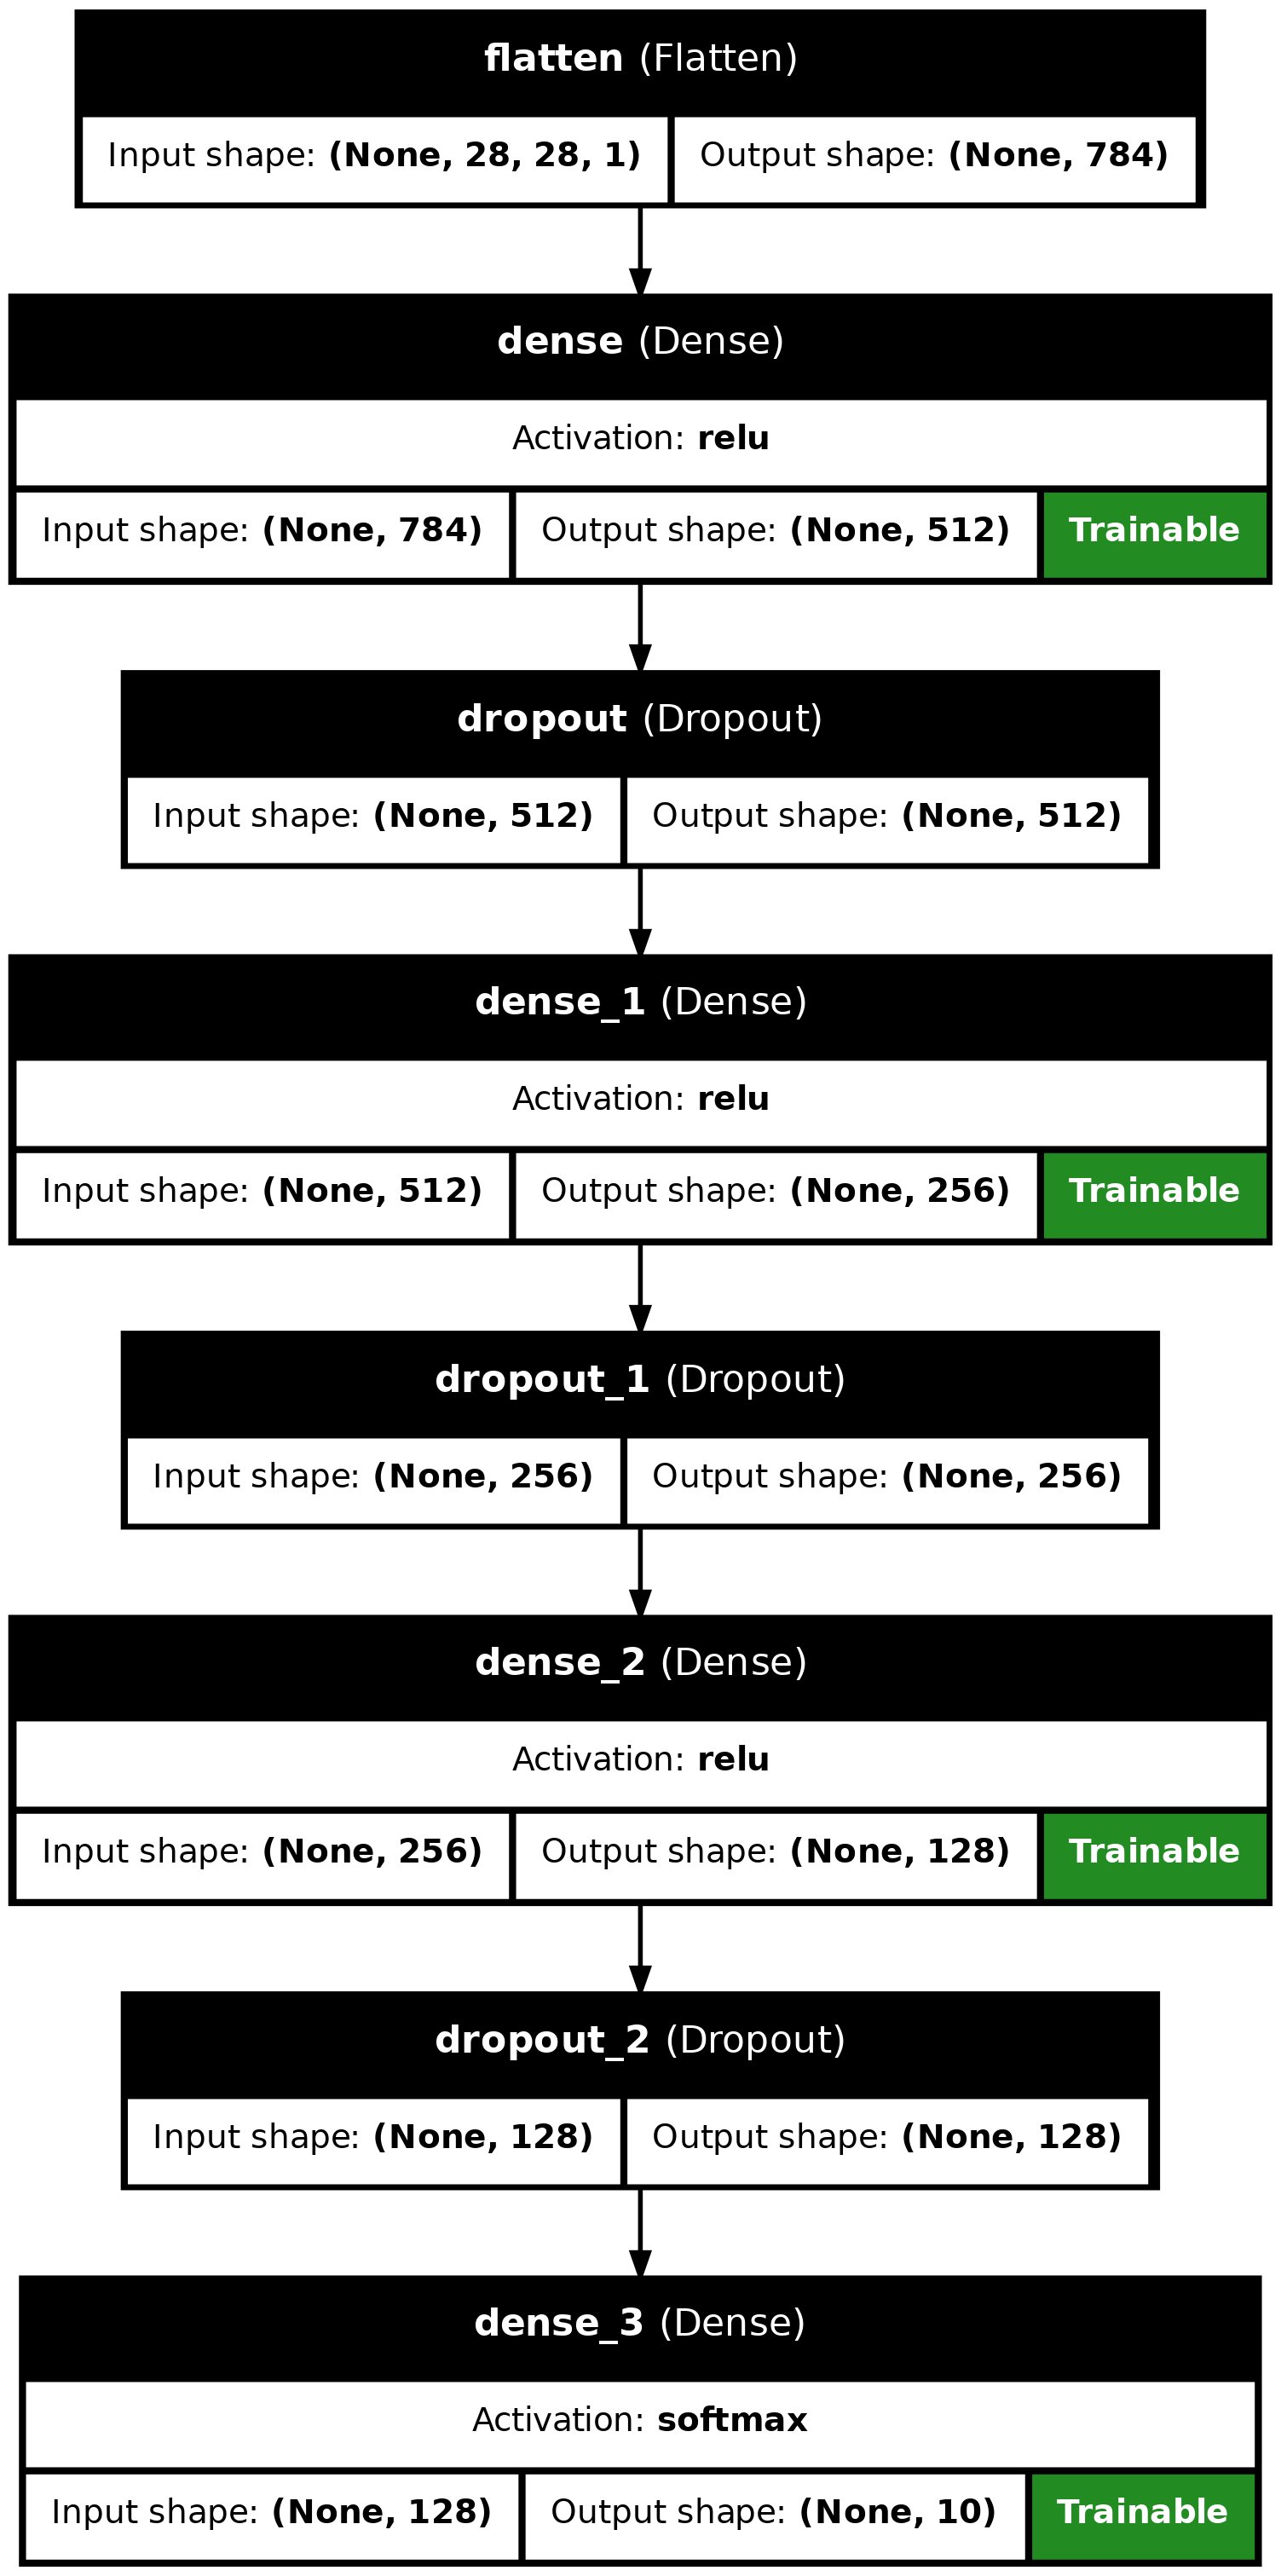
\includegraphics[width=\textwidth]{../images/models/model_fcnn_graph.png}
    \caption{Modelo FCNN}
    \label{fig:model_fcnn_graph}
  \end{minipage}
\end{figure}

Uma das exigências no enunciado é que o modelo FCNN e CNN tenham uma quantidade similar de parâmetros treinaveis. Assim sendo, o modelo FCNN (Figura \ref{fig:model_fcnn_graph}) possui 1333770 parâmtros treináveis, enquanto o modelo de CNN (Figura \ref{fig:model_cnn_graph}) possui 1199882 parâmetros treináveis.


Para realizar o treinamento, predição e outras tarefas relacionadas aos modelos anteriores, foi utilizado o tensorflow \cite{tensorflow2015-whitepaper} e keras \cite{chollet2015keras}.

Abaixo segue algumas configurações feitas nos modelos, fora as demostradas nas Figuras \ref{fig:model_cnn_graph} e \ref{fig:model_fcnn_graph}:

\begin{enumerate}
  \item \textbf{Early stopping:}Os modelos não possuem um número fixo de épocas para o treinamento, foi estabelecido um número arbitráriamente grande de 10 mil épocas e, quando o valor de loss na validação não diminui em 10 épocas seguidas o treinamento é parado e o melhor modelo escolhido é aquele que possui o menor valor de loss na validação. 
  \item \textbf{Reduce learning rate on plateu:} A taxa de aprendizado dos modelos inicia como 0.001, porém, quando o valor de loss na validação começa a ter poucas variações, essa taxa de aprendizado é reduzida. Isso faz com que os pesos mudem menos ao longo das épocas quando o treinamento está chegando em um mínimo, assim trazendo uma mais precisão. 
  \item \textbf{Função de loss:} A função de loss escolhida foi a \textit{categorical crossentropy}, pois dentro as funções de loss implementadas no keras é a que mais atendia as especificações do projeto.
  \item \textbf{Otimizador:} O otimizador escolhido foi o adadelta
\end{enumerate}


\subsection{Execução do código}

O código utilizado para gerar os resultados apresentados nesse relatório se encontra em um repositório do GitHub \footnote{https://github.com/semcovici/kmnist-classification} e as instruções para a execução se encontram no arquivo README.md na seção ``Instruções".


\section{Resultados}

Na tabela~\ref{table:results_f1}, temos os resultados de \textit{F1-Score} para cada uma das 10 classes no conjunto de teste, bem como o resultado de \textit{F1-Score macro} (média aritimética do \textit{F1-Score} das classes), que nos dá uma visão geral do desempenho do modelo para todas as classes.

\begin{table}[H]\scriptsize\centering
\begin{tabular}{l|rrrrr}
\toprule
classe & CNN & CNN com data augmentation & CNN sem polling & FCNN & FCNN com data augmentation \\
\midrule
0 & 0.9114 & 0.9508 & 0.9168 & 0.9127 & 0.9514 \\
1 & 0.8728 & 0.9042 & 0.8867 & 0.8778 & 0.9107 \\
2 & 0.8483 & 0.8850 & 0.8354 & 0.8409 & 0.8676 \\
3 & 0.9223 & 0.9259 & 0.9202 & 0.9260 & 0.9187 \\
4 & 0.8681 & 0.9034 & 0.8737 & 0.8739 & 0.9112 \\
5 & 0.9013 & 0.9263 & 0.8976 & 0.9074 & 0.9232 \\
6 & 0.8765 & 0.9272 & 0.8906 & 0.8890 & 0.8996 \\
7 & 0.9038 & 0.9444 & 0.9025 & 0.9008 & 0.9471 \\
8 & 0.8694 & 0.9170 & 0.8773 & 0.8763 & 0.9211 \\
9 & 0.9002 & 0.9388 & 0.9016 & 0.8994 & 0.9409 \\
\midrule
macro avg & 0.8874 & 0.9223 & 0.8902 & 0.8904 & 0.9192 \\
\bottomrule
\end{tabular}

    
\caption{Resultados de \textit{F1-Score} no conjunto de teste (arredondados em 4 casas decimais)}
\label{table:results_f1}
\end{table}

É possível ver que, em todos os modelos, o desempenho em cada classe é bastante consistente, não tenho classes que possuem uma grande vantagem em detrimento das outras e, também, não há classes em grande desvantagem. 

Considerando o \textit{F1-Score macro}, vemos que os diferentes experimentos não causaram grandes diferenças nos resultados, tendo o pior resultado sendo a CNN com 88.74\% de \textit{F1-Score macro} e o melhor sendo a CNN com data augmentation com 92.23\% de \textit{F1-Score macro}.

Remover a camada de polling traz ganhos aparentemente não significativos ao desempenho do modelo no conjunto de teste, tendo em vista que há uma diferença de aproximadamente 0.26\% nos resultados. Já a adição de \textit{data augmentation} se mostra eficiente na melhora do desempenho nos dois algoritmos testados, FCNN e CNN. 


Por outro lado, quando olhamos a curva de aprendizado da CNN (Figura \ref{fig:cnn_loss_progress}) e da FCNN (Figura \ref{fig:fcnn_loss_progress}), vemos que a CNN converge por volta de 600 épocas, enquanto a FCNN precisa de quase o dobro de épocas para convergir.

\begin{figure}[H]
\centering
\begin{minipage}{0.5\textwidth}
  \centering
  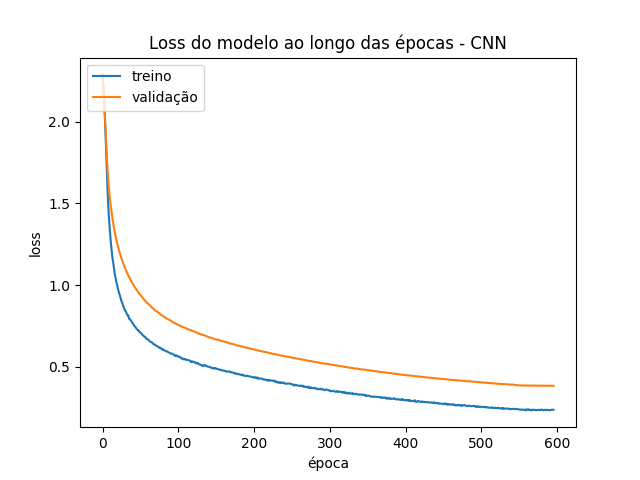
\includegraphics[width=\textwidth]{../images/results_plt/cnn_loss_progress.png}
  \caption{Curva de aprendizado CNN}
  \label{fig:cnn_loss_progress}
\end{minipage}%
\hfill
\begin{minipage}{0.5\textwidth}
  \centering
  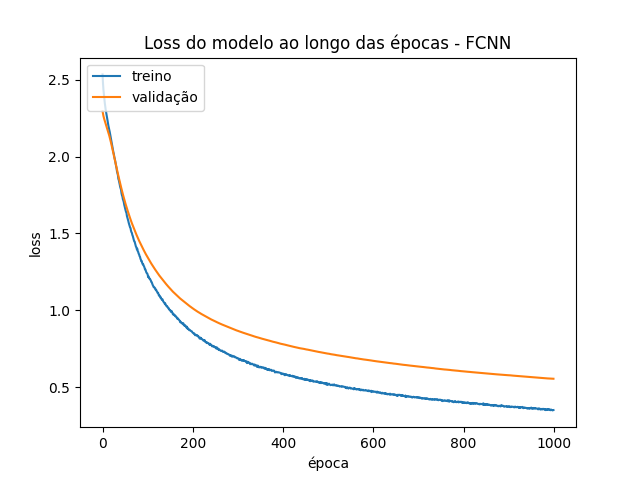
\includegraphics[width=\textwidth]{../images/results_plt/fcnn_loss_progress.png}
  \caption{Curva de aprendizado FCNN}
\label{fig:fcnn_loss_progress}
\end{minipage}
\end{figure}

Já a remoção da camada de polling da CNN faz o modelo convergir mais rápido, porém vemos um \textit{overfitting} do modelo no treino, tendo um loss menor que 0.25 no cojunto de treino no fim do treinamento, que é menor que o loss final do conjunto de treino na CNN tradicional, como demostrado na Figura \ref{fig:cnn_sem_polling_loss_progress}. 


\begin{figure}[ht]
  \centering
  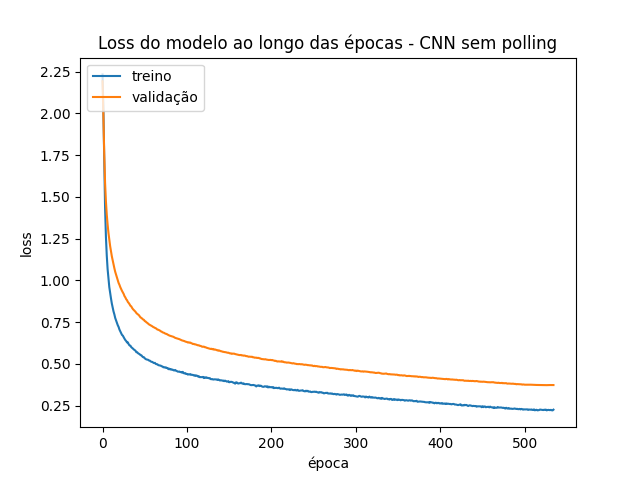
\includegraphics[width=.5\textwidth]{../images/results_plt/cnn_sem_polling_loss_progress.png}
  \caption{Curva de aprendizado CNN sem polling}
  \label{fig:cnn_sem_polling_loss_progress}
\end{figure}

A adição do \textit{data augmentation} na CNN traz uma redução drástica do \textit{overfitting} do modelo no treinamento, tendo o loss ao longo das épocas no treino e validação bem próximos, conforme demostrado na Figura \ref{fig:cnn_com_data_augmentation_loss_progress}. Já na FCNN a adição da etapa de data augmentation também traz uma redução no \textit{overfitting}, porém não tanto quando a CNN, conforme demostrado na Figura \ref{fig:fcnn_com_data_augmentation_loss_progress}. Além disso, a adição de \textit{data augmentation} mostra uma redução no número de épocas para convergir. Em contraponto a isso, a adição de mais dados faz com que seja mais custoso computacionamente treinar o modelo, de forma que a redução de épocas não diminui o tempo de treinamento. 

\begin{figure}[H]
  \centering
  \begin{minipage}{0.5\textwidth}
    \centering
    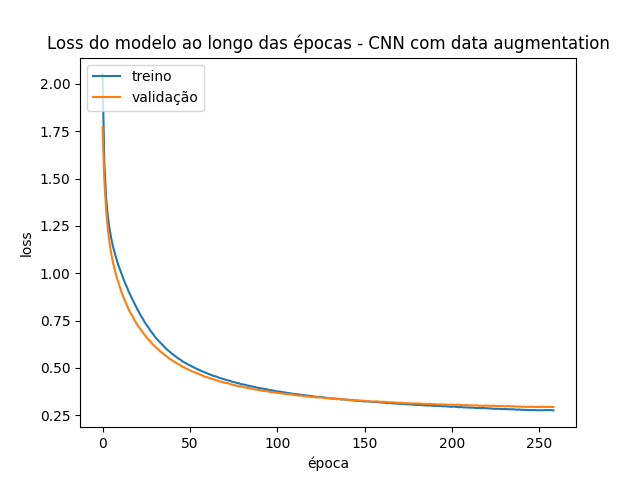
\includegraphics[width=\textwidth]{../images/results_plt/cnn_com_data_augmentation_loss_progress.png}
    \caption{Curva de aprendizado CNN com \textit{data augmentation}}
    \label{fig:cnn_com_data_augmentation_loss_progress}
  \end{minipage}%
  \hfill
  \begin{minipage}{0.5\textwidth}
    \centering
    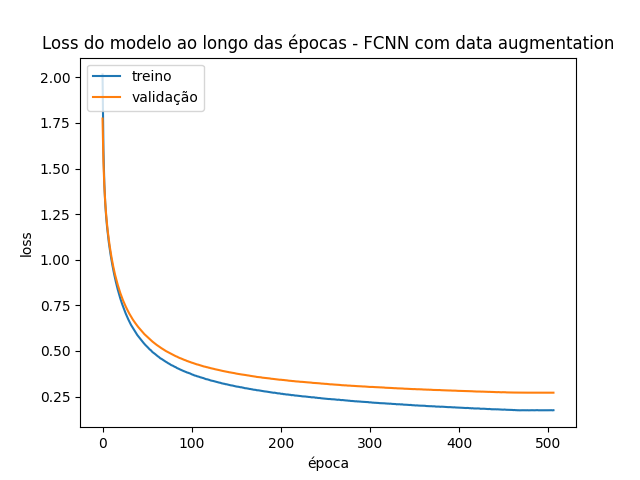
\includegraphics[width=\textwidth]{../images/results_plt/fcnn_com_data_augmentation_loss_progress.png}
    \caption{Curva de aprendizado FCNN com \textit{data augmentation}}
    \label{fig:fcnn_com_data_augmentation_loss_progress}
  \end{minipage}
\end{figure}


Nas Figuras \ref{fig:model_cnn_layer_0_kernel_plot} e \ref{fig:model_cnn_layer_1_kernel_plot}, temos os filtros formados após o treinamento do modelo CNN nas camadas convolucionais. Não há algum padrão interpretável nesses filtros que nos mostre algum aspecto que o modelo aprendeu nas imagens. Isso não significa que o modelo não aprendeu nada nas imagens, isso apenas significa que a análise dos filtros gerados não resulta em nenhum aspecto de melhor entendimento do funcionamento do modelo.  


\begin{figure}[H]
  \centering
  \begin{minipage}{0.5\textwidth}
    \centering
    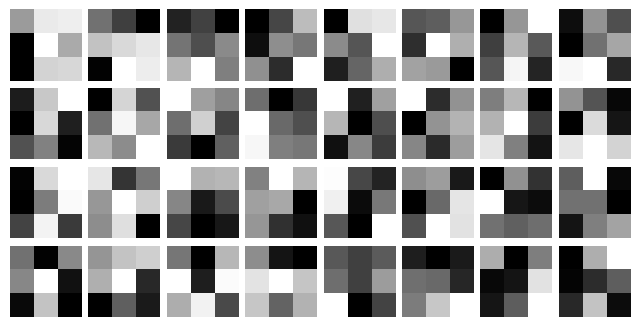
\includegraphics[width=.5\textwidth]{../images/kernels_plt/model_cnn_layer_0_kernel_plot.png}
    \caption{Filtros da primeira camada convolucional do modelo de CNN}
    \label{fig:model_cnn_layer_0_kernel_plot}
  \end{minipage}%
  \hfill
  \begin{minipage}{0.5\textwidth}
    \centering
    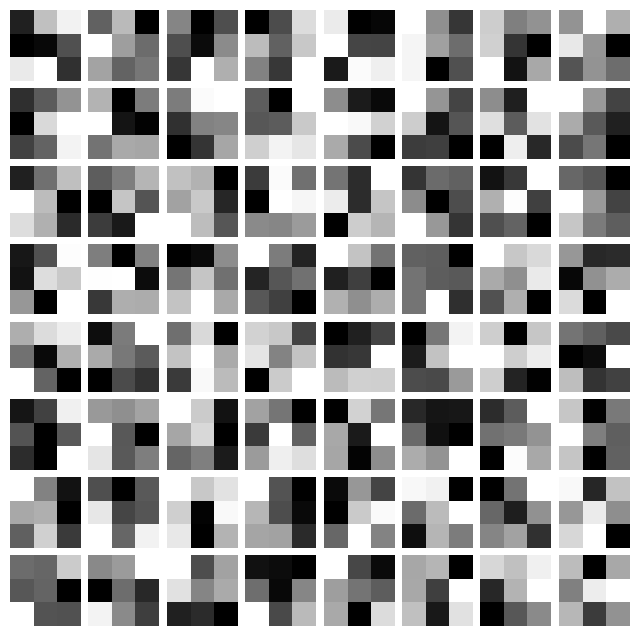
\includegraphics[width=.5\textwidth]{../images/kernels_plt/model_cnn_layer_1_kernel_plot.png}
    \caption{Filtros da segunda camada convolucional do modelo de CNN}
    \label{fig:model_cnn_layer_1_kernel_plot}
  \end{minipage}
  \end{figure}

  Esse padrão de ``filtros não interpretáveis" se repete  na versão sem camada de polling e na versão com \textit{data augmentation}.




\section{Conclusão e limitações}

\bibliographystyle{sbc}
\bibliography{sbc-template}

\end{document}
